\documentclass[09pt]{beamer}

\usetheme{Szeged}
\usecolortheme{rose}

\usepackage{color}
\usepackage{xcolor}
\usepackage{beamerthemeshadow}
\usepackage{mathrsfs}
\usepackage{url}
\usepackage{listings}
\usepackage{amssymb}

\definecolor{greenish}{RGB}{152,204,112}
\definecolor{redish}{RGB}{244,158,196}

\setbeamertemplate{navigation symbols}{}
\newcommand*{\LargerCdot}{\raisebox{-0.25ex}{\scalebox{3.0}{$\cdot$}}}
\expandafter\def\expandafter\insertshorttitle\expandafter{%
  \insertshorttitle\hfill%
  \insertframenumber}%\,/\,\inserttotalframenumber}


\begin{document}

\author{Kacper Sokol}
\title[Learning \texttt{Prolog} rules]{Learning \texttt{Prolog} rules \& \\extracting features from signals}
\institute{Department of Computer Science}
\titlegraphic{
\includegraphics[scale=.5]{../paper/gfx/UOB-logo}}
\date{\today}

\begin{frame}
\titlepage
\end{frame}

\begin{frame}
  \frametitle{Table of contents}
  \tableofcontents
\end{frame} 


\section{Background}

  \subsection{World's population}
  \begin{frame}[plain]
    \frametitle{Population ageing}
    \begin{figure}
      \centering
      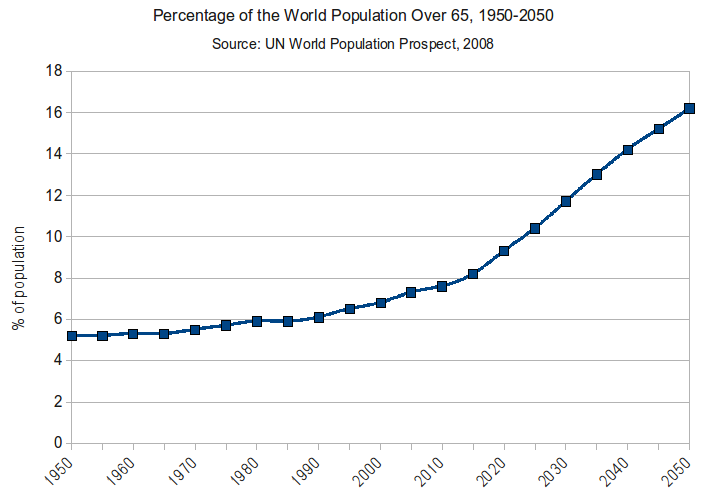
\includegraphics[scale=.4]{gfx/populationOver65}
      \caption{Percentage of world population over 65, 1950--2050; \cite{populationAgeing}}
    \end{figure}
  \end{frame}

  \subsection{SPHERE Project}
  \begin{frame}[allowframebreaks]
    \frametitle{SPHERE project~\cite{sphere}:\\An EPSRC Interdisciplinary Research Collaboration} % (IRC)
    \begin{block}{The Challenge}
      \begin{columns}
        \begin{column}{6cm}
          \begin{itemize}
            \item Global population health issues
            \item Ageing population
            \item Increasing healthcare costs
            \item Decreasing quality of life
          \end{itemize}
        \end{column}
        \begin{column}{4cm}
          \begin{figure}
            
\includegraphics[scale=.13]{gfx/sphere} 
          \end{figure}
          \end{column}
      \end{columns}
    \end{block}
    \pause
    \begin{block}{The Technology}
      \begin{itemize}
        \item Sensors development for smart house applications
        \item \textbf{Use acquired information} to identify medical or well-being issues: predict falls, detect strokes, analyse eating behaviour, and detect periods of depression or anxiety
      \end{itemize}
    \end{block}
    \pause
    \begin{block}{The Approach}
      Collaboration of clinicians, engineers, designers and social care professionals as well as members of the public to develop helpful technologies:
      \begin{itemize}
        \item Focus on real-world technologies acceptable in people's homes
        \item Address real healthcare problems in a cost effective way
      \end{itemize}
    \end{block}
  \end{frame}



\section{Applications}

\subsection{Spatio-temporal data}
\begin{frame}[fragile]
\frametitle{...Use acquired information...}
{\tiny
\begin{columns}
\begin{column}{5.4cm}
\begin{example}[\tiny Smart house output~\cite{cook2009assessing}]
\begin{figure}
\lstset{
captionpos=b,
% frame=single,
language=HTML,
breaklines=true,
% caption=CASAS dataset structure,
% label=lst:data,
float=tb,
basicstyle=\tiny
}
\begin{lstlisting}
...
2008-02-26 10:52:58.577436 M17   OFF
2008-02-26 10:52:59.792264 M17   ON
...
2008-02-26 10:53:43.512642 I02   ABSENT
2008-02-26 10:53:43.978491 I01   ABSENT
...
2008-02-26 10:53:52.112690 AD1-B 0.0421
2008-02-26 10:53:54.721822 M17   ON
...
\end{lstlisting}
\caption{\tiny CASAS experiment dataset structure\label{lst:data}}
\end{figure}
\end{example}
\end{column}
\pause
\begin{column}{5.4cm}
\begin{example}[\tiny Data transformation]
\begin{figure}
\lstset{
captionpos=b,
% frame=single,
language=HTML,
breaklines=true,
% caption=Learnt rules,
% label=lst:rules,
float=tb,
basicstyle=\tiny
}
\begin{lstlisting}
...
sensor(m09, false, relative, 4772648).
sensor(m09, false, absolute, 120411621).
sensor(m09, false, sequence, 9).
sensor(m09, false, windowed, 0).

sensor(i08, false, relative, 5692364).
sensor(i08, false, absolute, 120411622).
sensor(i08, false, sequence, 10).
sensor(i08, false, windowed, 1).
...
\end{lstlisting}
\tiny\caption{\tiny Knowledge representation\label{lst:knowledge}}
\end{figure}
\end{example}
\end{column}
\end{columns}
}
\end{frame}

\subsection{Goal}
\begin{frame}
  \frametitle{Extract knowledge}
  \begin{block}{Objectives}
    \begin{itemize}
      \item Learn activity recognition model
      \item Distinguish multiple occupiers
      \item Extract more informative signal features
    \end{itemize}
  \end{block}
  \pause
  \begin{block}{Challenges}
    \begin{itemize}
      \item Lack of labelled data to train and test models
      \item Incompleteness of data
      \item Noisy data
      \item Time handling (unbounded variable)
      \item Real valued sensor output
      \item Information loss: room and sensor layout
    \end{itemize}
  \end{block}
\end{frame}

\begin{frame}[fragile]
\frametitle{Output}
\begin{example}[Rules for activity recognition]
\begin{figure}
\lstset{
captionpos=b,
% frame=single,
language=HTML,
breaklines=true,
% caption=Learnt rules,
% label=lst:rules,
float=tb
}
\begin{lstlisting}
activity(Person, cooking, TimeWindow) :-
    location(Person, TimeWindow, kitchen),
    device(TimeWindow, hob).

location(Person, TimeWindow, kitchen) :-
    sensor(m08, on, absolute, TimeWindow),
    sensor(m09, on, absolute, TimeWindow).

device(TimeWindow, hob) :-
    sensor(ad1-a, on, absolute, TimeWindow).
\end{lstlisting}
\caption{Learnt rules\label{lst:rules}}
\end{figure}
\end{example}
\end{frame}  


\section{Techniques}

  \subsection{Inductive Logic Programming}
  \begin{frame}%[plain]
    \frametitle{Inductive Logic Programming (ILP)}
    \begin{block}{ILP~\cite{muggleton1994inductive,muggleton1995inverse}}
      \begin{itemize}
        \item Fusion of \emph{inductive learning} and \emph{logic programming} aiming at best of both worlds
        \item Powerful knowledge representation as \emph{first-order logical rules}
        \item Build model from available observations
        \item Generate new knowledge form experience
        \item Background knowledge incorporated into model
        \item Induction as a basic mode of inference: generalization of specific observations to theories
        \item Human readable model
      \end{itemize}
    \end{block}
  \end{frame}

  \begin{frame}%[plain]
    \frametitle{Power of ILP}
    \begin{block}{How does it work?}
        \begin{figure}
          \centering
          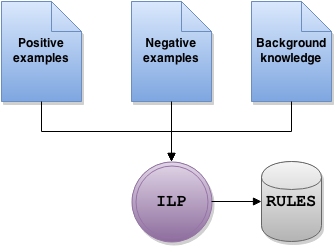
\includegraphics[scale=.5]{../paper/gfx/ilp}
          \caption{ILP scheme\label{fig:ilp}}
        \end{figure}
    \end{block}
  \end{frame}

  \subsection{ILP in healthcare}
  \begin{frame}
    \frametitle{Advantages}
    \begin{block}{Innovative?}
      \begin{itemize}
        \item Background knowledge: room and sensor layout, activity structure, etc.\
        \item First order logic---parametrised rules: more powerful than widely used propositional logic
        \item Human readable models easy to inspect and tune
      \end{itemize}
    \end{block}
    \pause
    \begin{block}{Suitable?}
      \begin{itemize}
        \item Use of background knowledge not contained in the dataset gives more power
        \item Customisable recognition model
        \item Possible to extend with \emph{Data Narrative}
      \end{itemize}
    \end{block}
  \end{frame}

\section{Contribution}

  \subsection{Challenges}
  \begin{frame}
    \frametitle{Challenges}
    \begin{itemize}
      \item \makebox[0pt][l]{$\square$}\raisebox{.15ex}{\hspace{0.1em}$\checkmark$} Design customisable spatio-temporal (smart house) data generator to test and design models
      \item \makebox[0pt][l]{$\square$}\raisebox{.15ex}{\hspace{0.1em}$\checkmark$} Investigate spatio-temporal data representation as logical facts
      \item \makebox[0pt][l]{$\square$}\raisebox{.15ex}{\hspace{0.1em}$\color{white}\checkmark$} Research representation of unbounded variables like time in first-order logic
      \item \makebox[0pt][l]{$\square$}\raisebox{.15ex}{\hspace{0.1em}$\color{white}\checkmark$} Examine use of background knowledge not contained in the original dataset
      \item \makebox[0pt][l]{$\square$}\raisebox{.15ex}{\hspace{0.1em}$\color{white}\checkmark$} Create and test different activity recognition models in ILP
      \item \makebox[0pt][l]{$\square$}\raisebox{.15ex}{\hspace{0.1em}$\color{white}\checkmark$} Build mechanism for new features discovery
    \end{itemize}
  \end{frame}

  \subsection{Deliverables}
  \begin{frame}%[plain]
    \frametitle{Deliverables}
    \begin{itemize}
      \item Easy to use spatio-temporal data generator
      \item Framework for spatio-temporal data analysis with ILP
      \item Limitations of ILP when applied to spatio-temporal data
      \item Methodology for time representation in knowledge form
      \item Evaluation of ILP model: contrast \& compare against widely used solutions
      \item Feature extraction mechanism
    \end{itemize}
  \end{frame}




\section*{}%References
  \begin{frame}[allowframebreaks,plain]
    \frametitle{References}
    \bibliographystyle{amsalpha}
    \bibliography{../paper/yhpargoil.bib,bg.bib}
  \end{frame}

  \begin{frame}[plain]
    \centering \Huge Q\&A \par
  \end{frame}

\end{document}
